\documentclass[border=10pt]{standalone}
\usepackage{xcolor}
\usepackage{tikz}
\usepackage{pgfplots}
\pgfplotsset{compat=1.18}

\definecolor{BG}{HTML}{FAFAFA}
\definecolor{INK}{HTML}{1A1A2E}
\definecolor{SUB}{HTML}{555566}
\definecolor{BAR}{HTML}{4361EE}
\definecolor{MARK}{HTML}{D81159}

\begin{document}
\pagecolor{BG}
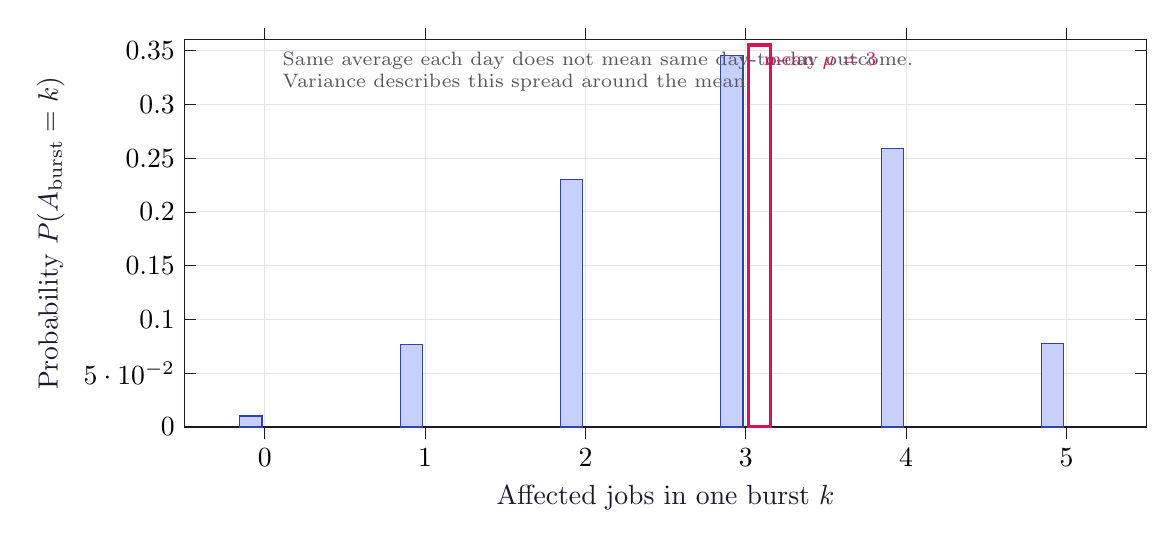
\begin{tikzpicture}
\begin{axis}[
  width=13.8cm,
  height=6.5cm,
  ybar,
  bar width=8pt,
  xlabel={Affected jobs in one burst \(k\)},
  ylabel={Probability \(P(A_{\mathrm{burst}}=k)\)},
  xmin=-0.5, xmax=5.5,
  ymin=0, ymax=0.36,
  xtick={0,1,2,3,4,5},
  ytick={0,0.05,0.10,0.15,0.20,0.25,0.30,0.35},
  grid=major,
  grid style={draw=gray!20},
  axis line style={draw=INK},
  tick style={draw=INK},
  xlabel style={text=INK},
  ylabel style={text=INK},
]
% Binomial(J_b=5, p=0.6)
\addplot[draw=BAR!70!black, fill=BAR!30] coordinates {
(0,0.01024)
(1,0.07680)
(2,0.23040)
(3,0.34560)
(4,0.25920)
(5,0.07776)
};
\addplot[MARK, very thick] coordinates {(3,0) (3,0.355)};
\node[font=\scriptsize, text=MARK, anchor=west] at (axis cs:3.05,0.34) {mean \(\mu=3\)};
\node[font=\scriptsize, text=SUB, align=left, anchor=west] at (axis cs:0.05,0.33)
{Same average each day does not mean same day-to-day outcome.\\Variance describes this spread around the mean.};
\end{axis}
\end{tikzpicture}
\end{document}
